En esta sección hablaremos acerca de lo que es el Centro Mexicano para la Producción más Limpia, cuál es su función como parte del IPN y las normas y procedimientos que lo rigen, así como la estructura interna que maneja para la realización y coordinación de sus diversas actividades.

\section{El Centro Mexicano para la Producción más Limpia del Instituto Politécnico Nacional}

	El Centro Mexicano para la Producción más Límpia (CMPL) es una instancia del Instituto Politécnico Nacional (IPN)que se dedica a la investigación y elaboración de procesos de producción más limpia. El CMPL, como dice en su página web:

	\begin{quotation}Es integrante de la red mundial de centros de producción más límpia y de la red latinoamericana de producción más limpia, promovidas por la Organización de las Naciones Unidas para el Desarrollo Industrial (ONUDI) y el Programa de las Naciones Unidas para el Medio Ambiente (PNUMA). Cuenta con 13 años de experiencia realizando trabajo técnico para la industria nacional atendiendo sectores como alimentos, petroquímicos, cementeros, galvanoplastia y embotelladoras, por mencionar algunos. Los servicios que ofrece el CMPL son: diagnóstico en producción más limpia y eficiencia energética, diplomados a distancia, presenciales y Maestría en Producción Más Limpia, realización de proyectos de mecanismo de desarrollo limpio, planes de manejo de residuos y análisis de químicos[1].
	\end{quotation}
	
	Con todo lo anterior, el CMPL requiere estar certificado por un Sistema Integral de Gestión para la Calidad y el Medio Ambiente, el cual se denomina SIG y que garantiza que el CMPL cumple con todos los lineamientos requeridos para ser considerado un centro de producción más limpia. El SIG está soportado por la normas ISO 9001 (para la calidad) y la norma ISO 14000 (para el medio ambiente). Es importante saber qué dicen estas normas y cómo son aplicadas dentro de los procedimientos y servicios del CMPL para entender la importancia de implementar un sistema de información que ayude a cumplir con dichas normatividades dentro del CMPL.\\
	
	\subsection{ISO 9001}
	La Norma ISO 9001:2008 elaborada por la Organización Internacional para la Estandarización (ISO), determina los requisitos para un Sistema de Gestión de la Calidad (SGC), que pueden utilizarse para su aplicación interna por las organizaciones, sin importar si el producto o servicio lo brinda una organización pública o empresa privada, cualquiera que sea su tamaño, para su certificación o con fines contractuales.\\
	
	La estructura que tiene esta norma se encuentra diseñada de la siguiente manera.\\
	
	\begin{itemize}
		\item Capítulo 1 al 3: Guías y descripciones generales.
		\item Capítulo 4 Sistema de gestión: contiene los requisitos generales y los requisitos para gestionar la documentación.
		\item Capítulo 5 Responsabilidades de la Dirección: contiene los requisitos que debe cumplir la dirección de la organización, tales como definir la política, asegurar que las responsabilidades y autoridades están definidas, aprobar objetivos, el compromiso de la dirección con la calidad, etc.
		\item Capítulo 6 Gestión de los recursos: la Norma distingue 3 tipos de recursos sobre los cuales se debe actuar: RRHH, infraestructura, y ambiente de trabajo. Aquí se contienen los requisitos exigidos en su gestión.
		\item Capítulo 7 Realización del producto/servicio: aquí están contenidos los requisitos puramente de lo que se produce o brinda como servicio (la norma incluye servicio cuando denomina "producto"), desde la atención al cliente, hasta la entrega del producto o el servicio.
		\item Capítulo 8 Medición, análisis y mejora: aquí se sitúan los requisitos para los procesos que recopilan información, la analizan, y que actúan en consecuencia. El objetivo es mejorar continuamente la capacidad de la organización para suministrar productos y/o servicios que cumplan con los requisitos.
	\end{itemize}
	
	El objetivo declarado en la Norma, es que la organización busque sin descanso la satisfacción del cliente a través del cumplimiento de los requisitos.\\
	
	Con la ISO 9001, el CMPL garantiza que sus procedimientos generen resultados basados en estándares internacionales, permitiendo así un mejor desarrollo de:\\

	\begin{itemize}
		\item Diagnósticos: El CMPL realiza visitas de reconocimiento a los clientes que deseen hacer sus procesos de producción de una forma más amigable con el medio ambiente, elaborando al final una propuesta técnico-económica que le permita eficientar sus procesos; si el cliente no está de acuerdo con los resultados entonces se cierra el diagnóstico, se presenta una nueva propuesta o se ofrecen otros servicios.
		\item Capacitaciones: El CMPL ofrece varios cursos de capacitación para manejo de residuos y químicos al sector público y privado, con el fin de promover la producción más limpia.
		\item Maestría de Producción más Limpia: El CMPL creó esta Maestría para formar especialistas que se involucren en el análisis de las etapas productivas de cualquier proceso, desde la selección de materias primas, insumos, tecnologías, hasta las emisiones contamintantes del proceso (líquidas, gases, residuos, etc.), así como los impactos ambientales de los productos y servicios.[2]
	\end{itemize}
	
	\subsection{ISO 14000}
	La norma ISO 14000 es un estándar internacional de gestión ambiental que se comenzó a publicar en 1996, tras el éxito de la serie de normas ISO 9000 para sistemas de gestión de la calidad. La norma ISO 14000 es una norma internacionalmente aceptada que expresa cómo establecer un Sistema de Gestión Ambiental (SGA) efectivo. La norma ISO 14000 va enfocada a cualquier organización, de cualquier tamaño o sector, que esté buscando reducir los impactos en el ambiente y cumplir con la legislación en materia ambiental.\\
	
	La norma ISO 14000 es un conjunto de documentos de gestión ambiental que, una vez implantados, afectará todos los aspectos de la gestión de una organización en sus responsabilidades ambientales y ayudará a las organizaciones a tratar sistemáticamente asuntos ambientales, con el fin de mejorar el comportamiento ambiental y las oportunidades de beneficio económico. Los estándares son voluntarios, no tienen obligación legal y no establecen un conjunto de metas cuantitativas en cuanto a niveles de emisiones o métodos específicos de medir esas emisiones. Por el contrario, ISO 14000 se centra en la organización proveyendo un conjunto de estándares basados en procedimientos y unas pautas desde las que una empresa puede construir y mantener un sistema de gestión ambiental.\\
	
	La norma se compone de 8 elementos, los mismos que se relacionan a continuación con su respectivo número de identificación:\\
	
	\begin{itemize}
		\item Sistemas de Gestión Ambiental (14001 Especificaciones y directivas para su uso – 14004 Directivas generales sobre principios, sistemas y técnica de apoyo).
		\item Auditorías Ambientales (14010 Principios generales- 14011 Procedimientos de auditorías, Auditorías de Sistemas de Gestión Ambiental- 14012 Criterios para certificación de auditores).
		\item Evaluación del desempeño ambiental (14031 Lineamientos- 14032 Ejemplos de Evaluación de Desempeño Ambiental).
		\item Análisis del ciclo de vida (14040 Principios y marco general- 14041 Definición del objetivo y ámbito y análisis del inventario- 1404).
	\end{itemize}

	Para apegarse esta norma, el CMPL cuenta con procedimientos para mitigar los impactos ambientales en la elaboración de todas sus actividades. Dichos procedimientos están divididos por subdirecciones y jefaturas, en un documento llamado "Manual de Procedimientos", en donde se describe, según ISO 14000, la forma en la que estas áreas del CMPL deben operar. Incluyen procedimientos para la reducción de papel en la elaboración de documentos escritos, cuándo se deben sacar copias de ellos o cuándo es más viable compartirlo por correo electrónico y otros medios informáticos; el tiempo de inactividad de los equipos de cómputo antes de entrar en modo de ahorro de energía; configuraciones recomendadas para ahorro de energía en impresoras, scanners, fotocopiadoras, cámaras de video, servidores, pantallas, televisiones, aire acondicionado, microondas, refrigerador, expendedor de agua, no breaks y sites; en otras palabras, todo lo relacionado a las diversas actividades del CMPL. En la siguiente sección se describirán dichas actividades.
	
\subsection{Actividades del CMPL}
	Como toda institución pública y privada, el CMPL debe tener una organización que le permita coordinar todas las actividades de manera que cumplan con lo establecido en el SIG. Su organización está establecida como en la figura \ref{organigrama}, que es una estructura jerárquica.\\
	
	\begin{figure}[htbp!]
		\centering
			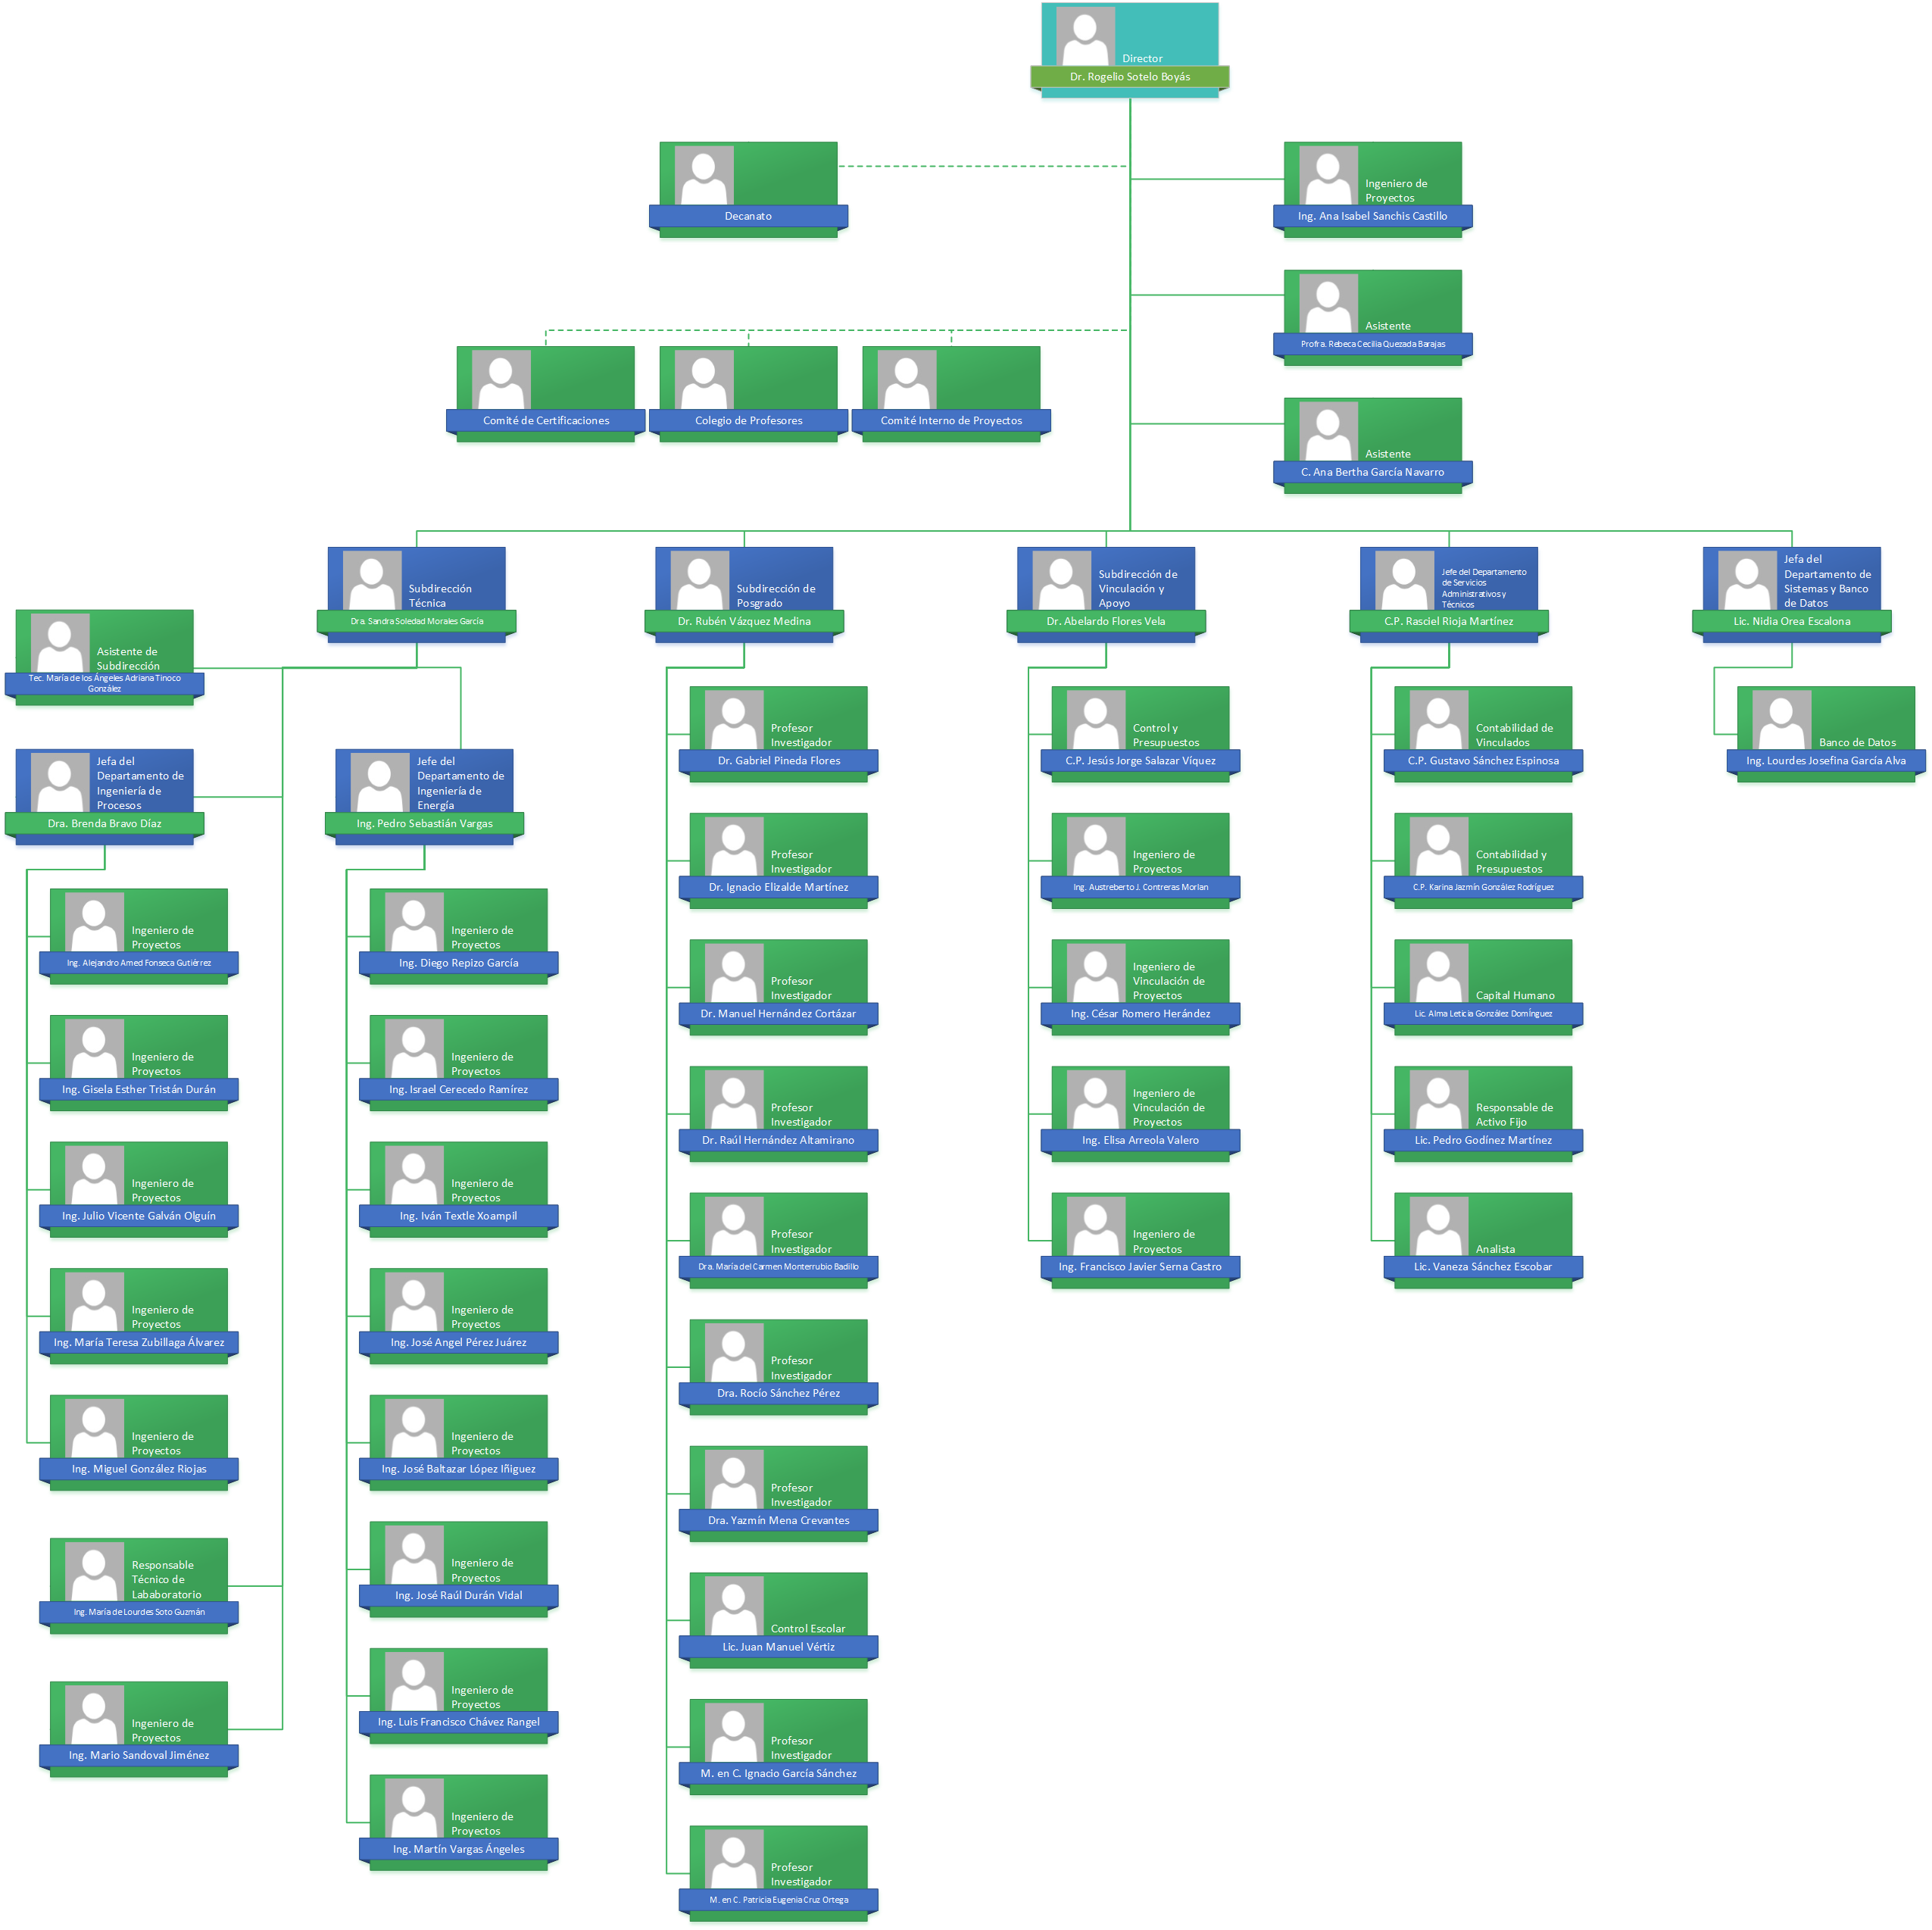
\includegraphics[width=1\textwidth]{images/antecedentes/OrganigramaCMPL.png}
		\caption{Diagrama de Estados de documentos entrantes.}
		\label{organigrama}
	\end{figure}
	
	El CMPL cuenta con una dirección, tres subdirecciones y cuatro departamentos, dos de los cuales están dentro de una subdirección. Cada subdirección y departamento debe entregar indicadores cada mes a la Dirección y una relación donde especifique los objetivos logrados durante el mes; esto con la finalidad de cumplir con la norma ISO 9001 para mejorar la calidad con la que el CMPL trabaja, buscando mejorarla con base en los indicadores de cada subdirección o departamento.\\
	
	Para que lo anterior sea posible, cada subdirección y departamento tiene sus manuales de procedimientos, mismos que deben ser revisados por la Dirección y que deben estar disponibles en todo momento para el personal administrativo y de apoyo del CMPL. La razón de llevar esto a cabo es que de cada subdirección y departamento se conozcan sus diversas actividades y funciones que tienen dentro del CMPL, de forma que se cumplan con sus objetivos de calidad, mismos que se enlistan a continuación.\\
	
	\begin{itemize}
		\item Dirección: Es la máxima autoridad en el CMPL. Aquí se decide qué se hace y el rumbo que toma el CMPL en función de los lineamientos que cada departamento o jefatura cumple con base en sus indicadores proporcionados cada mes.
		\item Subdirección Técnica: Realizar proyectos de Producción Más Limpia y Eficiencia Energética, que  ayuden a las empresas a prevenir y disminuir la generación de residuos, así como propiciar el uso eficiente de sus recursos.
		\item Subdirección de Vinculación y Apoyo: Los servicios del CMPL, realizar prospección para incrementar la cartera de clientes, así como establecer y mantener el contacto con los clientes.
		\item Subdirección de Posgrado: Formar recursos humanos en producción más limpia, eficiencia energética y otros temas relacionados con el desarrollo sustentable.
		\item Subdirección de Servicios Administrativos: Administrar los recursos asignados al CMPL.
		\item Departamento de Sistemas y Banco de Datos: Realizar el PEDMP y POA, así como sus seguimientos trimestrales. Coordinar las actividades de los RD's de los diferentes sistemas del CMPL.
	\end{itemize}
	
	Toda la información brindada por cada área demanda una cantidad considerable de materia de papelería, pues llevar todo ese proceso de forma manual hace que no se tenga un compromiso responsable con el medio ambiente.  Es en este proceso donde entra en juego la norma ISO 14000. Dicha norma exige al CMPL contar con un sistema computacional que automatice en gran parte los procesos del CMPL, buscando reducir la cantidad de papel utilizada, especialmente en documentos que son únicamente de carácter informativo.\\
	
	El Departamento de Sistemas y Banco de Datos había desarrollado anteriormente un sistema que alojaba de forma electrónica al SIG. Con este sistema se cumplía la reducción del papel y el uso de tecnologías de la información para tener un impacto ambiental más limpio en los procesos del CMPL  y así cubrir parte de los requisitos para obtener la certificación de la ISO 14000. El sistema llevaba como nombre “Intranet CMPL”, al ser una aplicación web que estaba alojada de forma local en la red del CMPL ,cuyas funciones eran:\\
	
	\begin{itemize}
		\item Alojar los manuales de procedimientos de cada subdirección y departamento del CMPL, incluyendo sus objetivos específicos y formatos propios de cada subdirección y departamento.
		\item Tener un registro del directorio del CMPL de forma global y por subdirección o departamento. 
		\item Alojamiento de indicadores mensuales por subdirección y departamento para su consulta en las auditorías internas y externas.
		\item Organigrama interno del CMPL.
		\item Formatos de adquisición y requisición de material diverso para el CMPL.
		\item Galería fotográfica con evidencia de los diferentes congresos, expediciones, proyectos y eventos en los que el CMPL ha sido partícipe.
		\item Directorio interno del CMPL.
		\item Sección de avisos de carácter público a todo el personal del CMPL. 
		\item Apartado de software institucional de producción y oficina.
		\item Formatos electrónicos diversos de documentos oficiales, memorándums, circulares y tripticos.
		\item Sección de artículos y reportajes de producción más limpia en el mundo.
		\item Programa de cursos, capacitaciones y servicios que presta el CMPL.
		\item Catálogo de precios de servicios.
		\item Galería de logos oficiales de dependencias con las que el CMPL trabaja.
		\item Control de correspondencia (oficios y memorándums).
	\end{itemize}
	
	Este sistema estaba alojado en un servidor del CMPL, curas características eran:
	
	\begin{itemize}
		\item Disco duro de 500 GB.
		\item Memoria RAM de 4 GB.
		\item Sistema Operativo Windows Server 2003.
		\item Servidor web IIS 4.0.
		\item ASP.NET.
		\item Microsoft Office Access 2000.
	\end{itemize}
	
	%Sin embargo, hubo un cambio de administración en el CMPL y a este sistema se le dejó de dar mantenimiento, volviéndose obsoleto y poco seguro con el tiempo, obligando al nuevo personal del CMPL a realizar todas sus actividades de forma manual, incumplimiento con la norma ISO 14000, causando que no recibieran dicha certificación en 2014, razón por la cual se pensó en volver a desarrollar un nuevo sistema que alojara al SIG y así poder seguir estando certificados por ISO 14000, que es de vital importancia para el CMPL.
	
	En abril del 2014 el CMPL tuvo un cambio de administración y en dicho suceso se perdió gran parte del SIG. Esta pérdida de información y recursos causó que el SIG quedara inservible para su aplicación en el CMPL, obligando al nuevo personal del CMPL a realizar todas sus actividades de forma manual, generando una serie de complicaciones que dieron paso a los problemas que se describen en el siguiente capítulo.